%必要事項
%論文に目を通す
%追加すべき事項
% - Deconv(CNN)
% - 誤差逆伝播?
% - バッチ
% - ? Adamの説明
\chapter{背景:ニューラルネットワーク}

本章では、教師あり学習の説明を行った後、本論文で必要となるニューラルネットワークの説明を行う。

\section{教師あり学習}

教師あり学習とは、学習データとして説明変数と対応するべき目的変数のペアが与えられる機械学習の手法である。また、機械学習とは、学習データに含まれる特徴をコンピュータプログラム~(モデル)~が自動で学習し、学習したモデルを用いて何らかの問題を解く手法のことである。

\subsection{教師あり学習の目的}

$X,Y$をそれぞれ説明変数と目的変数の集合とすると、$f:X\rightarrow Y$のうち任意の$\boldsymbol{x} \in X$について正しい値$\boldsymbol{y} \in Y$を出力する関数$f^{'}$を表現するモデルを作成することが教師あり学習の目的である。

また、$f(\boldsymbol{x})$の$f^{'}(\boldsymbol{x})$への近似の程度を評価する関数を損失関数$L$と呼ぶ。損失関数$L$は$L:Y \times Y \rightarrow \mathbb{R}^+$として定義され、値が小さいほど近似の程度が良い関数である。$\mathbb{R}^+$は非負の実数を表す。

ここで、モデルのパラメータを$\theta$とすると、$\theta$が実行可能解で損失関数の期待値を返す関数が目的関数となる最適化問題として教師あり学習を捉えることができる。また、この時の最適解$\theta^{'}$により定まる関数が$f^{'}$であり、目的関数は\ref{eq:SL0}として定式化される。

\begin{align}
    \label{eq:SL0}
    \mathbb{E}[L(\boldsymbol{y},f(\boldsymbol{x},\theta))]
\end{align}

\subsection{教師あり学習モデルの学習と汎化}

任意の$\boldsymbol{x}$と対応する$\boldsymbol{y}$の組を用意することは現実的には難しい。したがって、学習データのみでの最適化問題を解いて最適解として$\hat{\theta}$を求めることが教師あり学習モデルの学習の目標である。

しかし、$\hat{\theta}$により定まる$\hat{f}$は$f^{'}$に一致するとは限らない。従って、$\hat{f}$の$f^{'}$への近似の程度を評価する必要がある。そこで、学習データとは別のデータ~(評価データ)~を用意し、評価データについての損失関数の期待値を求めるなどにより未知のデータへのモデルの性能~(汎化性能)~を評価する。

%ここで改ページ
\clearpage

\section{MLP}

MLP~(Multilayer~perceptron)~はニューラルネットワークの一つであり、教師あり学習の手法として用いられる。また、ニューラルネットワークとは、神経細胞と神経細胞間のシナプス結合を通る電気信号により実現される脳の機能に類似した数理モデルの総称である。

\subsection{MLPと脳機能の関係}
\label{sec:neuron}

MLPでは、神経細胞を\prettyref{fig:neuron}のような人工ニューロンとして表現する。この人工ニューロンでは、樹状突起からの入力を$x_i$として表し、神経細胞間の結合強度を重み$W_i$として表し、活動電位の非線形な発生を活性化関数$\theta$として表し、神経細胞の活動電位の発生の閾値を調整するオフセットをバイアス項$b$として表す。そして、$W_i$を重みとした$x_i$の重み付き和に$b$を加えた値に活性関数$\theta$を作用させた出力$y$を返す。つまり、\prettyref{eq:MLP0_0}として定式化される。

\begin{align}
    \label{eq:MLP0_0}
    y=\theta(\sum_{i=1}^{m} W_{i} \times x_i+b)
\end{align}

%ここの表現
活性化関数としてはReLU関数~(\prettyref{eq:ReLU})~やSigmoid関数~(\prettyref{eq:Sigmoid})~などの非線形関数が選ばれる。また、誤差逆伝播法を用いるために、一般には活性化関数に微分可能な関数を選ぶ。

\begin{align}
    \label{eq:ReLU}
    \theta_{ReLU}(x)&=max(0,x)\\
    \label{eq:Sigmoid}
    \theta_{Sigmoid}(x)&=\frac{1}{1+e^{-x}}
\end{align}

\begin{figure}[b]
\centering
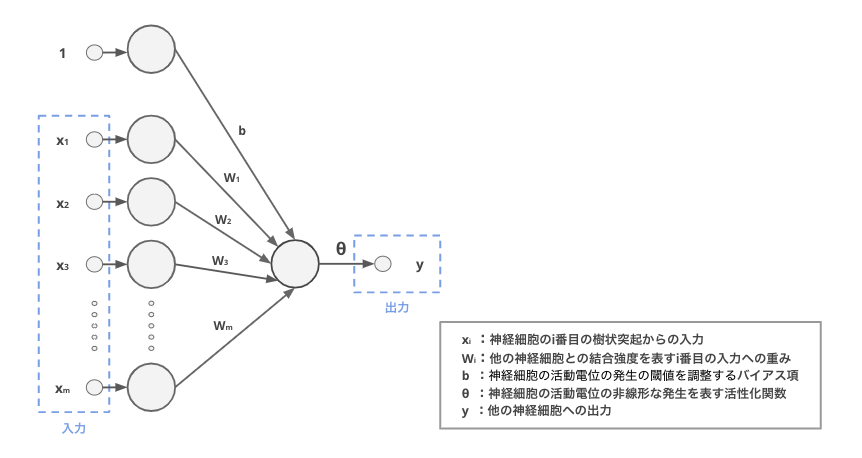
\includegraphics[width=0.5\hsize]{figure/neuron.png}
\caption[MLPの人工ニューロン]{人工ニューロン}
\label{fig:neuron}
\end{figure}

%ここで改ページ
\clearpage

\subsection{MLPの構造と定式化}

MLPは、\prettyref{sec:neuron}に示す人工ニューロンが複数並んだ層~(\prettyref{fig:MLP_net0})~により構成され、順伝播型の層構造のニューラルネットワークを形成する~(\prettyref{fig:MLP_net1})~。また、層構造は入力層と中間層と出力層を持ち、入力層と出力層はそれぞれ一層のみである。そして、層を構成する人工ニューロンの出力は次の層の全ての人工ニューロンに渡されるため、MLPを構成する層を全結合層と呼ぶ。

この時、\prettyref{eq:MLP0_0}を元にしてMLPの一層の出力$\boldsymbol{y}$は\prettyref{eq:MLP0_1}として導出される。$\boldsymbol{x},\boldsymbol{y},\boldsymbol{b}$は第$i$成分が層の$i$番目の人工ニューロンに対応するベクトルであり、それぞれ入力、出力、バイアス、である。そして、$W$は$(i,j)$成分が層の$j$番目の人工ニューロンの$i$番目の出力の重みに対応する重み行列であり、活性化関数$\theta$はそれぞれの出力に対して同様に作用する。

\begin{align}
    \label{eq:MLP0_1}
    \boldsymbol{y}=\theta(W\boldsymbol{x}+\boldsymbol{b})
\end{align}

\prettyref{eq:MLP0_1}より、MLPは\prettyref{eq:MLP0_2}として定式化される。また、$n$は層数であり、下付きの数字は何番目の層であるかを表す。

\begin{align}
    \label{eq:MLP0_2}
    \boldsymbol{y}=\theta_{n}(W_{n}(\theta_{n-1}(W_{n-1}\cdots(\theta_{1}(W_{1}\boldsymbol{x}+\boldsymbol{b_{1}}))\cdots+\boldsymbol{b_{n-1}}))+\boldsymbol{b_{n}})
\end{align}

\begin{figure}[b]
\centering
\begin{minipage}{0.4\hsize}
\centering
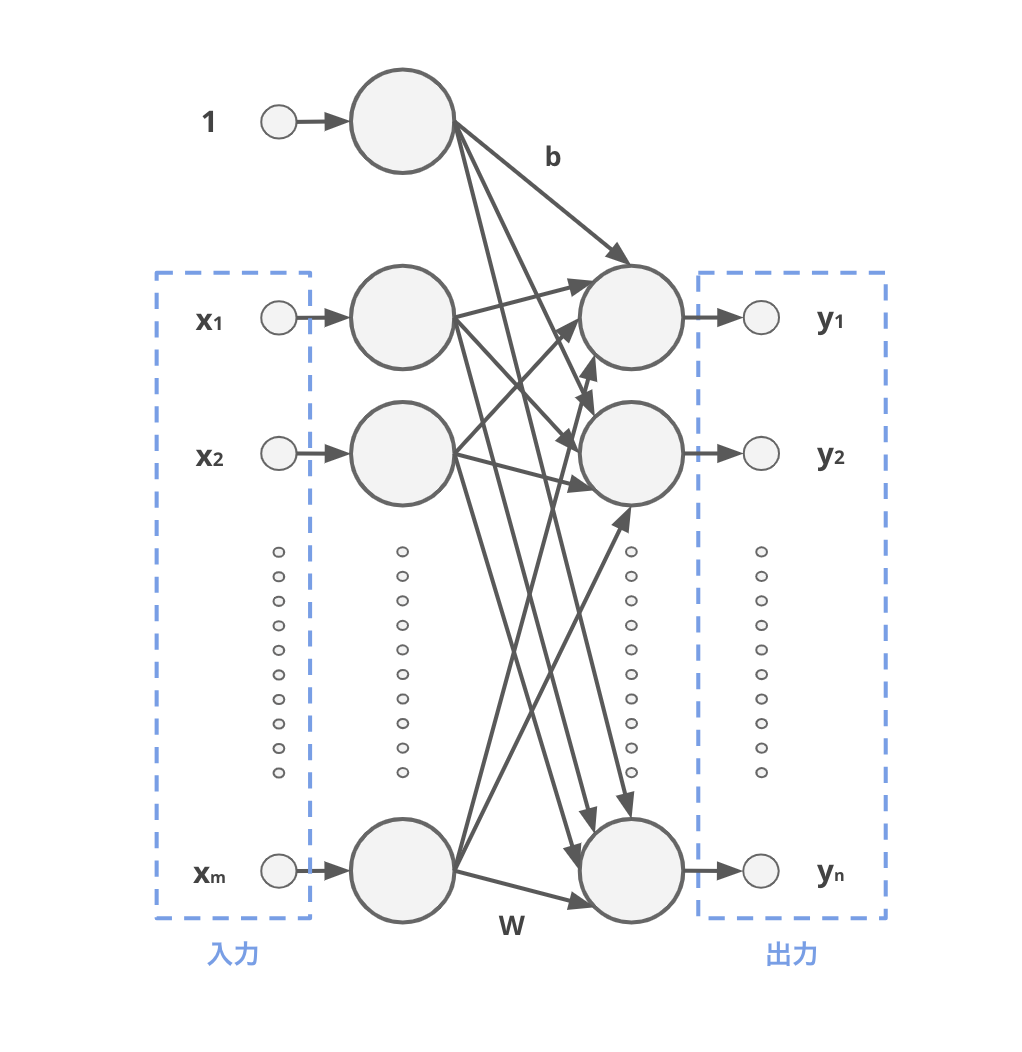
\includegraphics[width=0.95\hsize]{figure/mlp_net0.png}
\caption{MLPの一層}
\label{fig:MLP_net0}
\end{minipage}
\begin{minipage}{0.55\hsize}
\centering
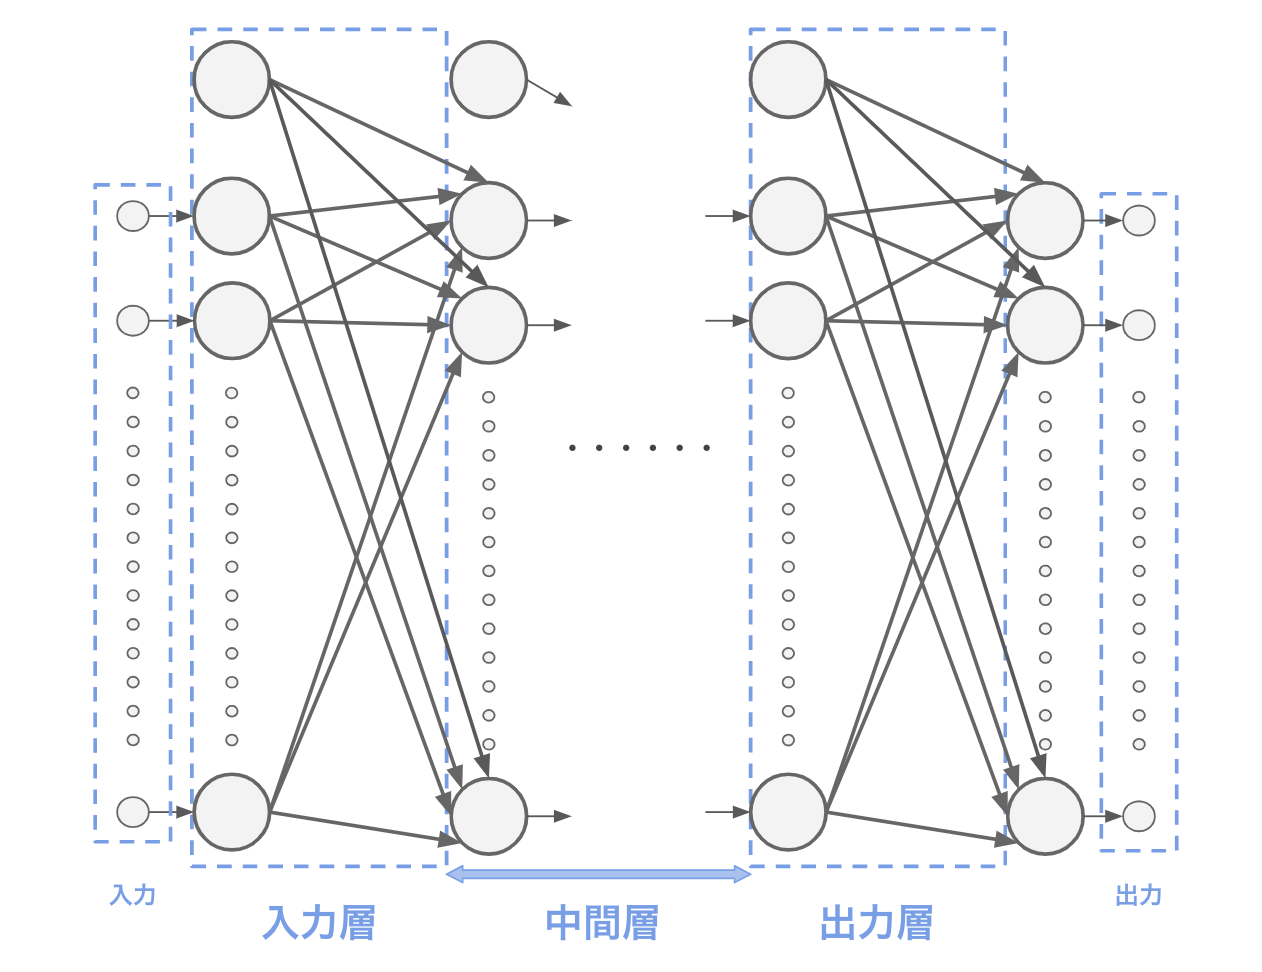
\includegraphics[width=0.9\hsize]{figure/mlp_net1.png}
\caption{MLPのネットワーク}
\label{fig:MLP_net1}
\end{minipage}
\end{figure}

%ここで改ページ
\clearpage

\subsection{MLPの学習}

MLPでは、説明変数と目的変数を実ベクトルに変換した後に学習を行う。また、実行可能解はパラメータである$W_i,\boldsymbol{b_i}$であり、最適解を求めるためにそれぞれ更新を行う。この時、損失関数$L$の勾配を用いた最適化アルゴリズム~(勾配降下法)~を一般には用いる。

\subsubsection{最急降下法}

最急降下法は最も急な降下方向である勾配の反対方向へのパラメータの更新を行う勾配降下法のアルゴリズムである。また、$W_i,\boldsymbol{b_i}$は\prettyref{eq:MLP2_0}及び\prettyref{eq:MLP2_1}にしたがって更新される。ここで、$\eta$は学習率と呼ばれる任意の正の実数であり、更新の程度を指定する。

\begin{align}
    \label{eq:MLP2_0}
    W _i &\leftarrow W_i - \eta \frac{\partial L}{\partial W_i} \\
    \label{eq:MLP2_1}
    \boldsymbol{b _i} &\leftarrow \boldsymbol{b_i} - \eta \frac{\partial L}{\partial \boldsymbol{b_i}}
\end{align}

\subsubsection{Adam}
\label{sec:Adam}

Adamは勾配降下法の中で最も用いられるアルゴリズムであり、\prettyref{alg:Adam}に示す手順にしたがってパラメータの更新を行う。アルゴリズムの詳細については~\cite{Adam}を参考にされたい。

\begin{algorithm}[b]
\label{alg:Adam}
    \DontPrintSemicolon
    \SetKwInOut{KwHyParam}{HyperParameter}
    \SetKwInOut{KwParam}{Parameter}
    \SetKwInOut{KwObFunc}{Objective~Function}
    \KwHyParam{$\beta_1,\beta_2\in \interval[open left]{0}{1},\eta,\epsilon$}
    \KwObFunc{$f$}
    \KwParam{$\theta$}
    \Init{
        \settowidth{\maxwidth}{$m_1,m_2 \leftarrow 0,0$~}
        \algalign{$t \leftarrow 0$~}{(Initialize~timestep)\;}
        \algalign{$\theta \leftarrow \theta_0$~}{(Initialize~Parameter)\;}
        \algalign{$m_1,m_2 \leftarrow 0,0$~}{(Initialize~moments)\;}
    }
    \Proc{
        \While{$\theta$ not converged}{
            \settowidth{\maxwidth}{$m_1,m_2 \leftarrow \beta_1 \cdot m_1+(1-\beta_1) \cdot g,\beta_2 \cdot m_2+(1-\beta_2) \cdot (g \odot g)$~}
            \algalign{$t \leftarrow t+1$~}{(Update~timestep)\;}
            \algalign{$g \leftarrow \nabla _{\theta} f(\theta)$~}{(Compute~gradient~of~$f(\theta)$)\;}
            \algalign{$m_1,m_2 \leftarrow \beta_1 \cdot m_1+(1-\beta_1) \cdot g,\beta_2 \cdot m_2+(1-\beta_2) \cdot (g \odot g)$~}{(Update~biased~moments)\;}
            \algalign{$\hat{m_1},\hat{m_2} \leftarrow m_1/(1-\beta_1^t),m_2/(1-\beta_2^t)$~}{(Update~bias-corrected~moments)\;}
            \algalign{$\theta \leftarrow \theta - \eta \cdot \hat{m_1}/(\sqrt{\hat{m_2}}+\epsilon)$~}{(Update~Parameter)\;}
        }
        \Return{$\theta$}\;
    }
\caption{Adamの疑似コード}
\end{algorithm}

%ここで改ページ
\clearpage

\subsubsection{誤差逆伝播法}

%Bishop本に書いてある

勾配降下法においてはそれぞれのパラメータについて勾配を求める必要がある。この時、高速に勾配を求める方法として誤差逆伝播法が一般に用いられる。誤差を求める際は入力層から出力層の方向で計算を行うが~(順伝播)~、誤差逆伝播法では誤差を出力層から入力層の方向に伝えていく~(逆伝播)~。




\subsubsection{バッチ処理}
%誤差逆伝播



%ここで改ページ
\clearpage

\section{CNN}

CNN~(Convolution~Neural~Network)~は、MLPにおいて全結合層を畳み込み層とプーリング層の繰り返し構造に置換した順伝播型のニューラルネットワークである。著名な例としてAlexNet~\cite{AlexNet}と略されるCNNがあり、画像認識の大規模な競技会であるILSVRCで2位以下に10\%以上の認識精度の差をつけて優勝した~(2012年)~。AlexNetでは様々な工夫を行っているもののネットワーク構造は単純である。具体的には、\prettyref{fig:Alex}のように5層の畳み込み層と3層の全結合層から構成され、畳み込み層のうち3層では直後にプーリング層を入れている。

\subsection{CNNの構造}

CNNはネオコグニトロン~\cite{neocognition}を起源に持ち、脳の視覚野の機能を模倣するようなネットワーク構造を持つ。また、脳の視覚野には主に二つの機能がある。一つ目は刺激の位置により異なった位置のニューロンの活動電位が発生することであり、二つ目は視覚情報の特徴を段階的に受容することである。この二つの機能を畳み込み層とプーリング層によりCNNは表現する。

まず、畳み込み層では、人工ニューロン間の結合を局所領域に限定することで局所領域の特徴を抽出する。したがって、局所領域間の位置関係は変わらないため、前者の機能を模倣することができる。そして、プーリング層では、局所領域の人工ニューロンの出力をまとめることで局所領域の特徴を集約する。したがって、層を進むにつれて高段階の特徴が残るため、後者の機能を模倣することができる。

さらに、CNNはMLPと比べてパラメータ数を減少させることができる。なぜなら、MLPの全結合層では入力の人工ニューロン数と出力の人工ニューロン数の積が一層のパラメータ数となるが、CNNの畳み込み層ではカーネルに含まれるパラメータ数のみが一層のパラメータ数となるからである。また、CNNのプーリング層でも局所領域の人工ニューロンの出力をまとめることで特徴量マップのサイズが小さくなるため、パラメータ数の減少に大きく寄与する。ここで、特徴量マップとはそれぞれの層の入力から得られる出力をまとめたもののことである。

\begin{figure}[b]
\centering
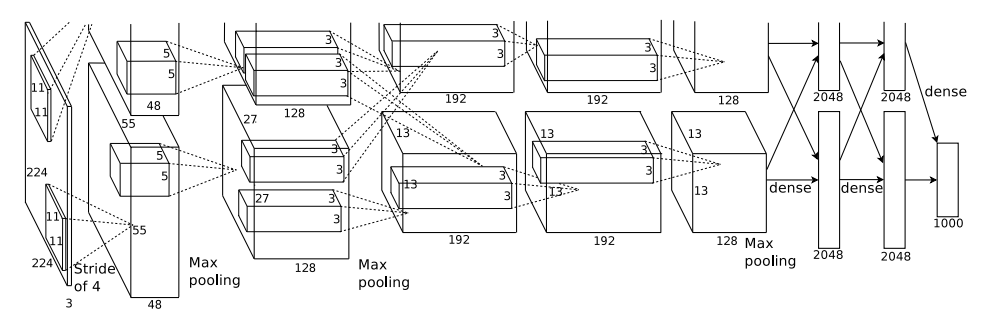
\includegraphics[width=\hsize]{figure/alex.png}
\caption{AlexNetのネットワーク}
\label{fig:Alex}
\end{figure}

%ここで改ページ
\clearpage

\subsection{畳み込み層}

畳み込み層においては、カーネルと呼ばれるフィルターを一定の間隔~(ストライド)~でスライドさせながらフィルターにより覆われた入力の部分の畳み込み演算を順に行う。畳み込み演算により、カーネルのそれぞれの値を重みとした対応する入力の部分の重み付き和を計算する。また、入力と出力の大きさを変えないために、一般には入力の周りに適当な幅で値を埋める操作を行う~(パディング)~。そして、画像のような二次元データにおいては、畳み込み演算は\prettyref{fig:conv}のように表現することができる。

さらに、入力を$I_h \times I_w$の行列、カーネルを$F_h \times F_w$の行列、ストライドを$S_h,S_w$、パディング幅を$P_h,P_w$、出力を$O_h \times O_w$の行列、とすれば、\prettyref{eq:conv}が成り立つ。\prettyref{fig:conv}においては、$I_h=I_w=4,F_h=F_w=3,S_h=S_w=1,P_h=P_w=1$であるため、$O_h=IO_w=4$となる。

\begin{align}
    \label{eq:conv}
    O_{h}&=\frac{I_h+2 P_h-F_{h}}{S_h}+1 \\
    O_{w}&=\frac{I_w+2 P_w-F_{w}}{S_w}+1
\end{align}

また、上記では入力と出力がいずれもチャンネル数が1つの場合を考えたが、実際には複数存在することが多い。したがって、カーネルの数は(入力チャンネル数)$\times$(出力チャンネル数)である。また、それぞれの出力チャンネル数に対し特徴量マップが入力チャンネル数だけ存在するが、これらの和にバイアス項を加えたものが実際の出力となる。

\begin{figure}[b]
\centering
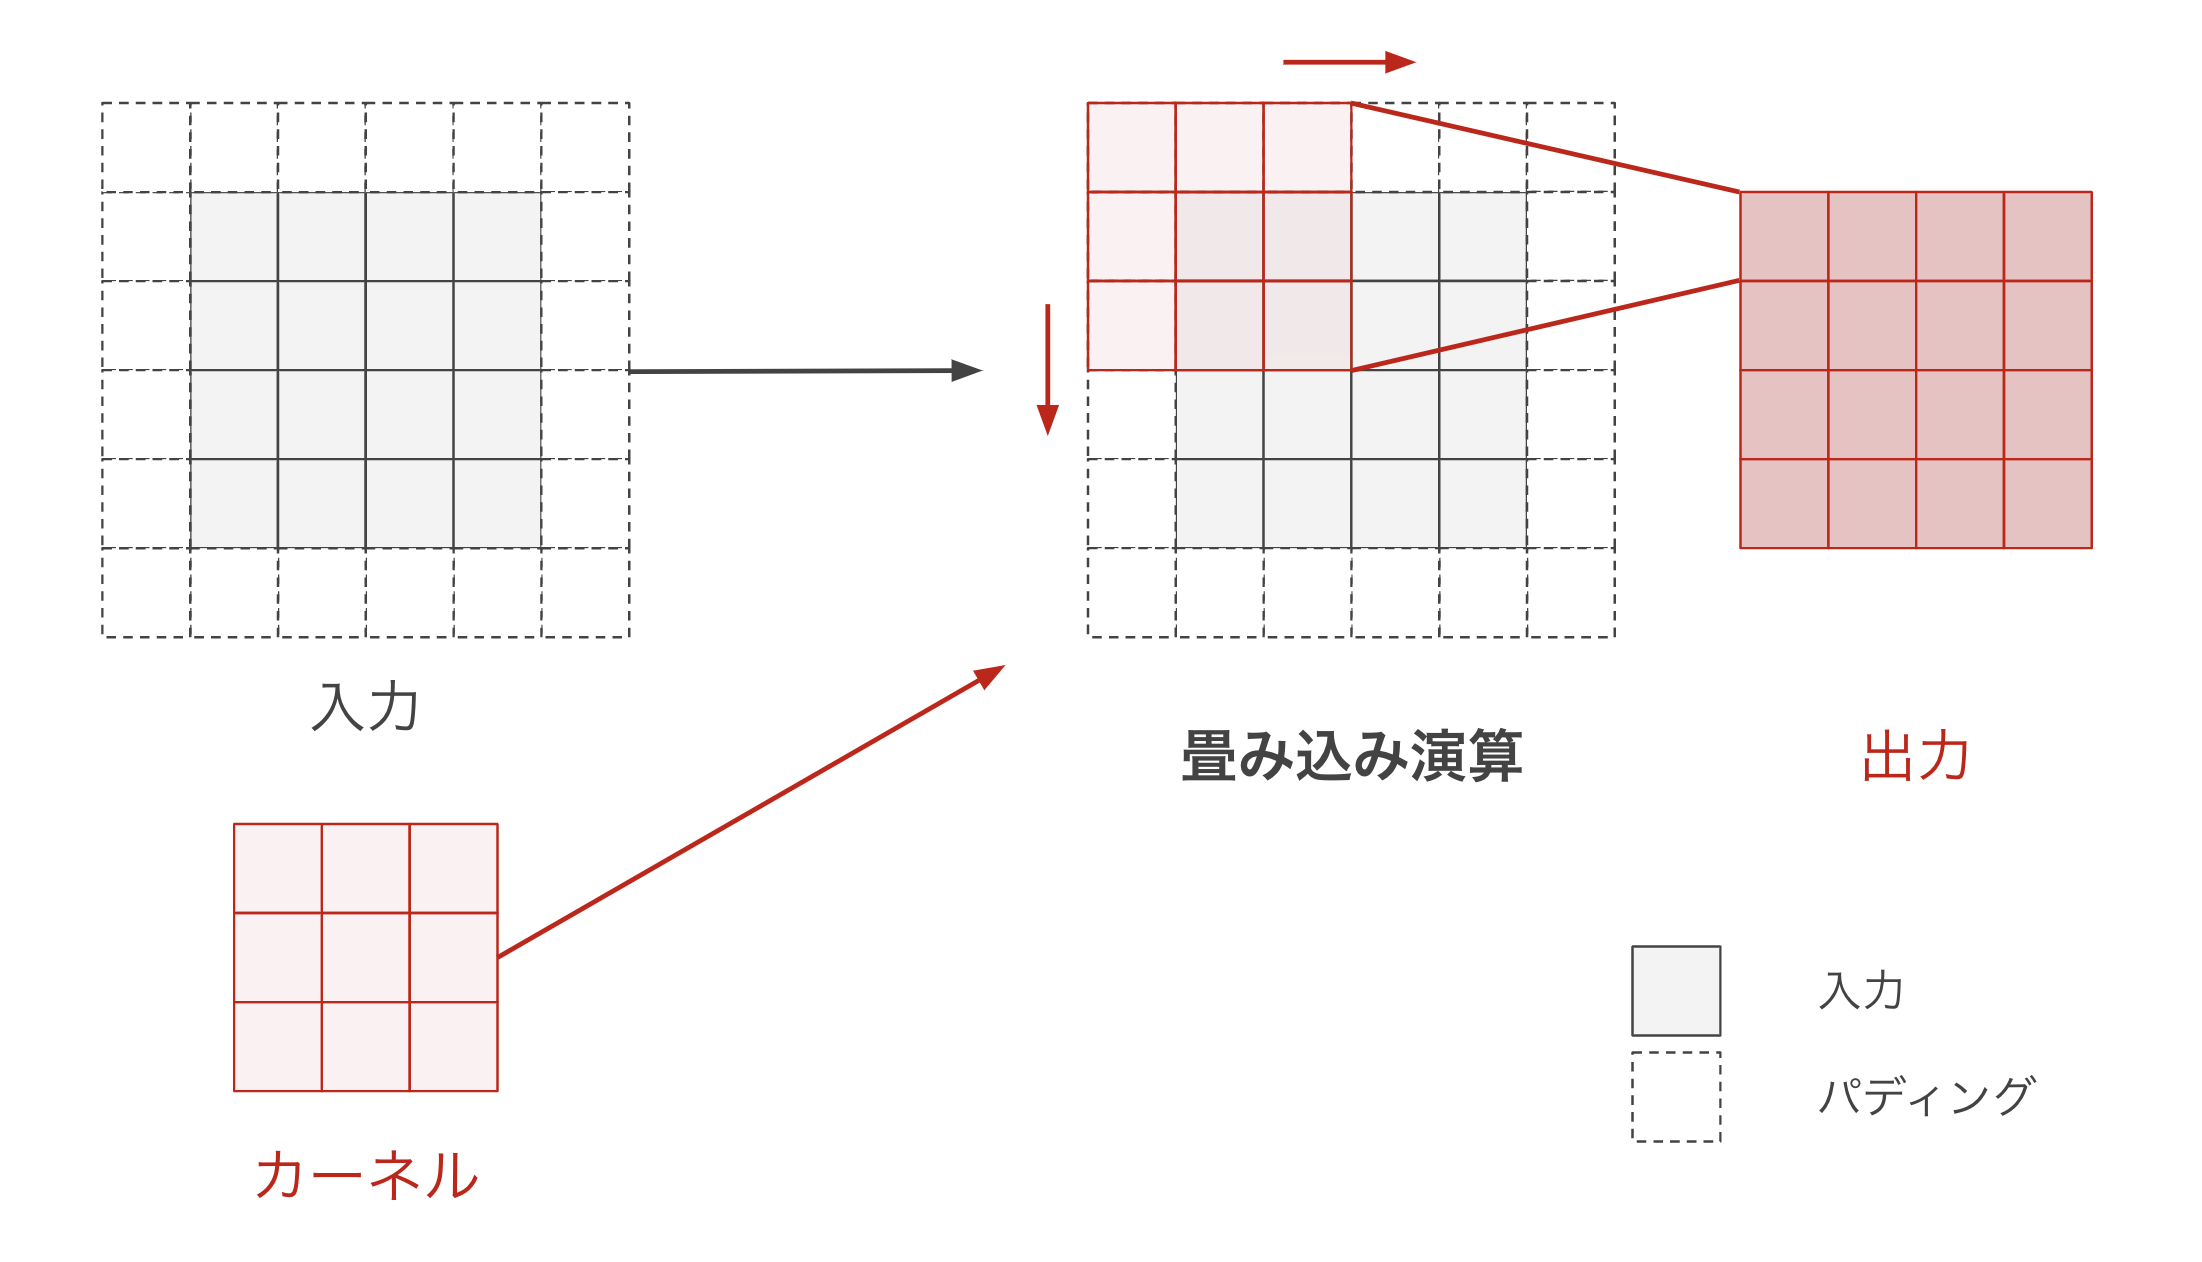
\includegraphics[width=\hsize]{figure/convolution.png}
\caption[CNNの畳み込み層]{畳み込み層\\
図は~\cite{AlexNet}のFigure~2を転載した。}
\label{fig:conv}
\end{figure}

%ここで改ページ
\clearpage

\subsection{プーリング層}

プーリング層においては、入力を局所領域ごとに分解し、領域ごとへの何らかの操作により情報量の圧縮を行う~(サブサンプリング、ダウンサンプリング)~。また、この時の操作で最大値をとる場合はMax~Pooling、平均値をとる場合はAverage~Poolingと呼び、主にこの二つが用いられる。

\begin{figure}[b]
\centering
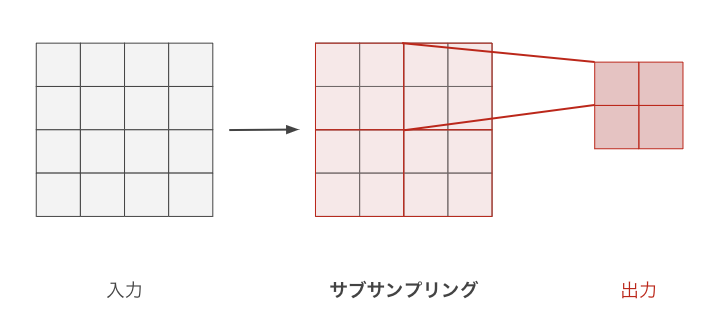
\includegraphics[width=\hsize]{figure/pooling.png}
\caption[CNNのプーリング層]{プーリング層}
\label{fig:pooling}
\end{figure}

%ここで改ページ
\clearpage

\section{GAN}

\begin{figure}[b]
\centering
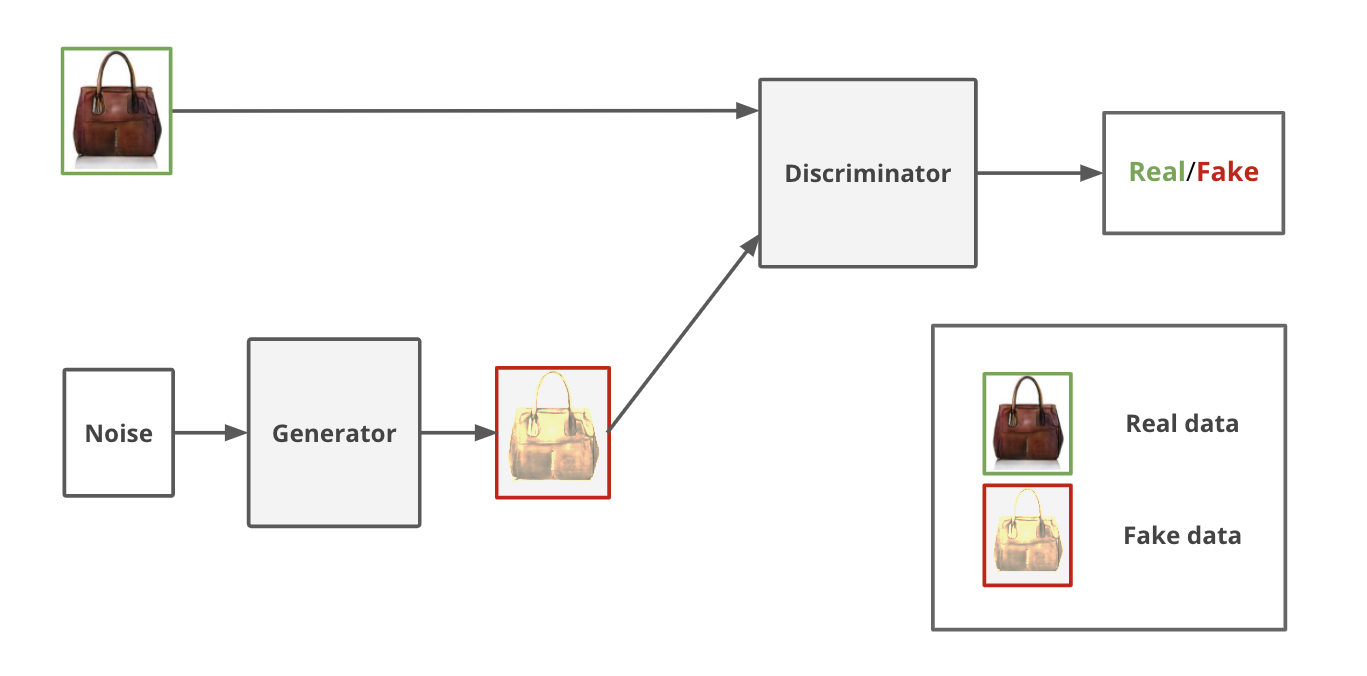
\includegraphics[width=\hsize]{figure/GAN_net.png}
\caption[GANのネットワーク]{GANのネットワーク\\
図は~\cite{pix2pix}のFigure~1を用いて作成した。}
\label{fig:GAN_net}
\end{figure}

GAN~(Generative~Adversarial~Networks)~\cite{GAN}はニューラルネットワークの応用例であり、学習データの特徴を持つ擬似的なデータを生成することを目指す手法である。この手法は実在しないアイドルの写真を生成する際などに用いられる~\cite{idol}。また、GANは\prettyref{fig:GAN_net}のように二つのニューラルネットワークで構成され、それぞれのネットワークはDiscriminator~(識別モデル)~とGenerator~(生成モデル)~と呼ばれる。

\subsection{GANの学習}

生成モデルと識別モデルの二つのネットワークはランダムに初期化された後に競合的に学習を進める。まず、識別モデルはデータがFake~data~(生成モデルの出力)~とReal~data~(学習データ)~のどちらであるかを識別できるように学習を進める。そして、生成モデルは識別モデルが学習データであると誤って識別するように、Noise~(ノイズ)~を元に学習データに近いデータを出力する。この二つの学習を交互に繰り返すことで、漸進的に生成モデルが学習データにより近いデータを生成できるようになると期待される。また、ノイズは適当な次元のベクトルであり、生成モデルの出力の揺らぎを表現する潜在変数の役割を果たす。

%ここで改ページ
\clearpage

\subsection{GANの定式化}

GANでは、生成モデルの目的関数は\prettyref{eq:GAN_G}、識別モデルの目的関数は\prettyref{eq:GAN_D}として定式化される。

\begin{align}
    \label{eq:GAN_G}
    \argmin _{\theta_G}& \mathbb{E}_{\boldsymbol{z}}[\log (1-D(G(\boldsymbol{z};\theta_G);\theta_D))]\\
    \label{eq:GAN_D}
    \argmax _{\theta_D}& \mathbb{E}_{\boldsymbol{x}}[\log D(\boldsymbol{x};\theta_D)]+\mathbb{E}_{\boldsymbol{z}}[\log (1-D(G(\boldsymbol{z};\theta_G);\theta_D))]
\end{align}


ここで、$\boldsymbol{x}$は学習データ、$\boldsymbol{z}$は生成モデルへの入力のノイズ、$G(\boldsymbol{z};\theta_G)$はノイズ$\boldsymbol{z}$を入力とする生成モデル、$D(\cdot;\theta_D)$は識別モデル、$\theta_G$は生成モデル$G$のパラメータ、$\theta_D$は識別モデル$D$のパラメータ、である。

\section{Pix2pix}

Pix2pix~\cite{pix2pix}は、ネットワークの入力に変換元の画像を~Condition~(条件)~として与えることで画像の変換を行うGANである~(\prettyref{fig:pix2pix_net})~。特定の条件をネットワークの入力に与えるGANとしてはConditional~GAN~(CGAN)~\cite{CGAN}が初めて考案されたが、Pix2pixは与えられた条件画像の構造を維持したまま変換するという点でCGANとは異なる。具体的には、線画から写真への変換や白黒画像からカラー画像への変換をPix2pixにより行うことができる~(\prettyref{fig:pix2pix_img})~。

\begin{figure}[b]
\centering
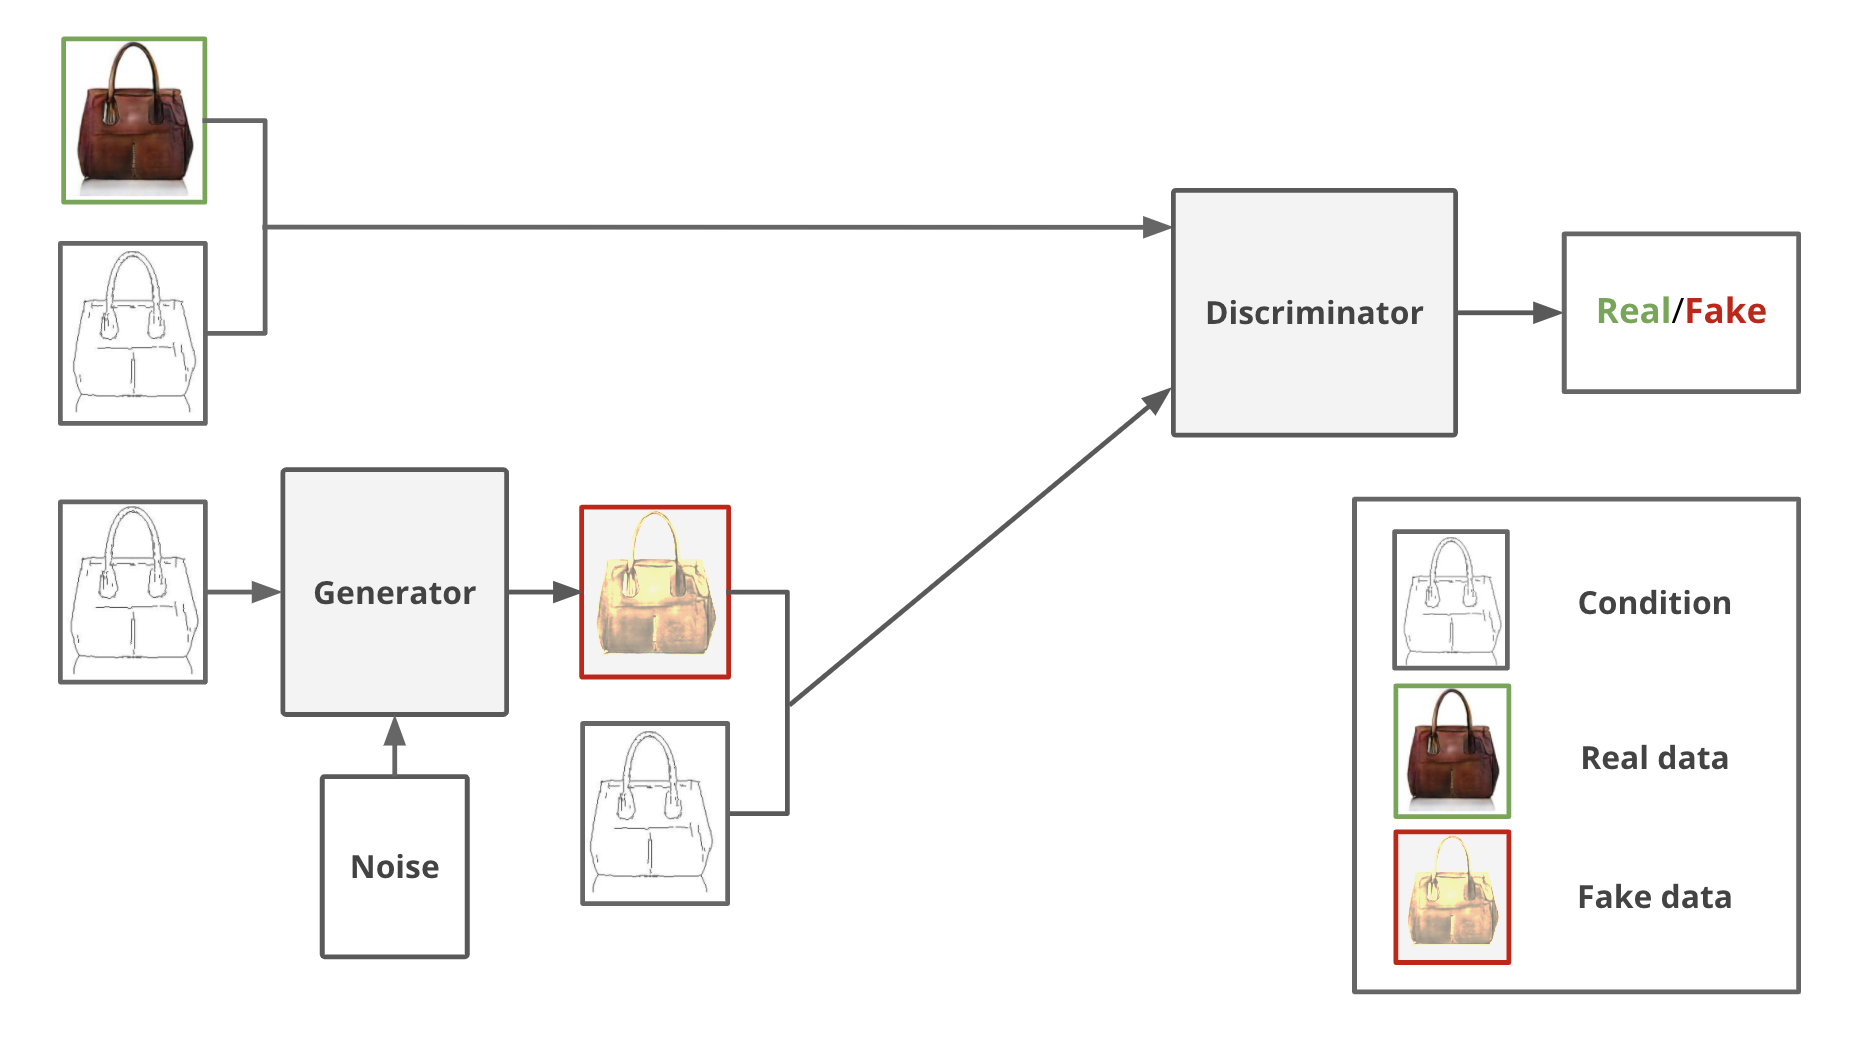
\includegraphics[width=0.9\hsize]{figure/pix2pix_net.png}
\caption[Pix2pixのネットワーク]{Pix2pixのネットワーク\\
図は~\cite{pix2pix}のFigure~1を用いて作成した。}
\label{fig:pix2pix_net}
\end{figure}

%ここで改ページ
\clearpage

\begin{figure}[t]
\centering
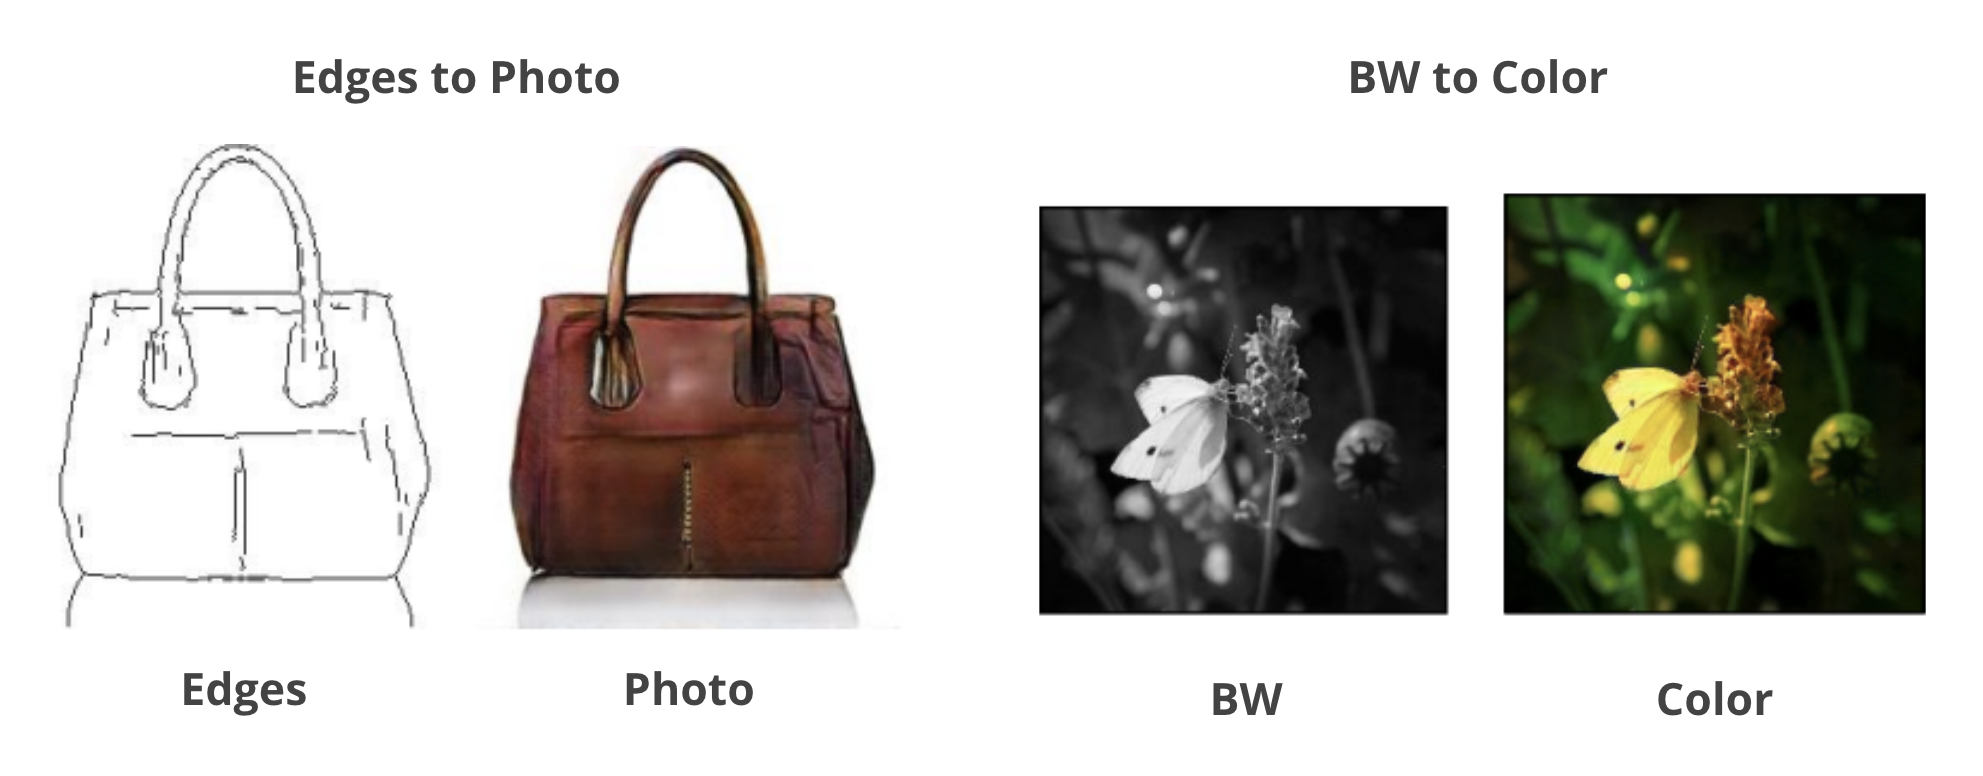
\includegraphics[width=\hsize]{figure/pix2pix_img.png}
\caption[Pix2pixのスタイル変換の例]{Pix2pixのスタイル変換の例\\
図は~\cite{pix2pix}のFigure~1を用いて作成した。}
\label{fig:pix2pix_img}
\end{figure}

\subsection{Pix2pixの定式化}

そして、Pix2pixにおいては、生成モデルの目的関数は\prettyref{eq:pix2pix_G}、識別モデルの目的関数は\prettyref{eq:pix2pix_D}として定式化される。

\begin{align}
    \label{eq:pix2pix_G}
    \argmin _{\theta_G}& \mathbb{E}_{\boldsymbol{y}, \boldsymbol{z}}[\log (1-D(\boldsymbol{y}, G(\boldsymbol{y}, \boldsymbol{z}; \theta_G); \theta_D))]+\mathbb{E}_{\boldsymbol{x}, \boldsymbol{y}, \boldsymbol{z}}[\|\boldsymbol{x}-G(\boldsymbol{y}, \boldsymbol{z}; \theta_G)\|_{1}]\\
    \label{eq:pix2pix_D}
    \argmax _{\theta_D}& \mathbb{E}_{\boldsymbol{x}, \boldsymbol{y}}[\log D(\boldsymbol{x}, \boldsymbol{y}; \theta_D)]+\mathbb{E}_{\boldsymbol{y}, \boldsymbol{z}}[\log (1-D(\boldsymbol{y}, G(\boldsymbol{y}, \boldsymbol{z}; \theta_G); \theta_D))]
\end{align}

ここで、$\boldsymbol{x}$は変換先の学習データ、$\boldsymbol{y}$は変換元の学習データ、$\boldsymbol{z}$は生成モデルへの入力のノイズ、$G(\boldsymbol{y},\boldsymbol{z};\theta_G)$は$\boldsymbol{y}$を条件としノイズ$\boldsymbol{z}$を入力とする生成モデル、$D(\boldsymbol{y},\cdot;\theta_D)$は$\boldsymbol{y}$を条件とする識別モデル、$\theta_G$は生成モデル$G$のパラメータ、$\theta_D$は識別モデル$D$のパラメータ、である。

\subsection{Pix2pixの生成モデル}

Pix2pixの生成モデルには、\prettyref{fig:u-net}のようにEncoder-Decoder型のネットワークが用いられる。ただし、変換元の画像と返還後の画像で共通する基本構造であるピクセルの対応関係を維持するために、スキップコネクションが用いられる。このスキップコネクションはU-net~\cite{u-net}で用いられたものと同様の働きをする。具体的には、エンコード前の特徴量マップをデコード時にも利用しており、この特徴量マップによりピクセルの対応関係が維持されると期待される。

また、ノイズとしては通常のGANのようなベクトルではなくDropout~\cite{Dropout}が用いられる。Dropoutとは、ニューラルネットワークの重みの更新の際にランダムにいくつかの重みを0として無視する手法のことである。

%ここで改ページ
\clearpage

\begin{figure}[t]
\centering
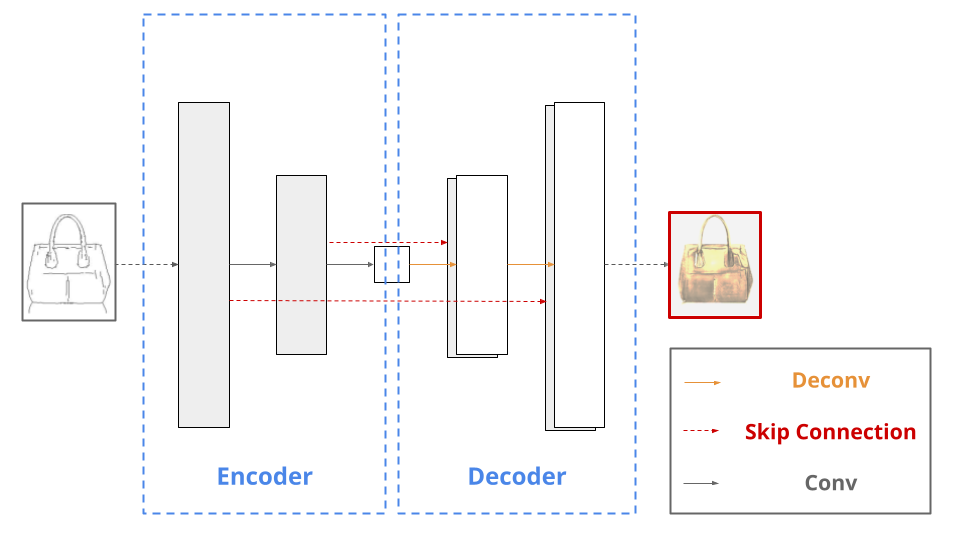
\includegraphics[width=0.8\hsize]{figure/u-net.png}
\caption[Pix2pixの生成モデル]{生成モデルのネットワーク\\
図は~\cite{pix2pix}のFigure~1とFigure~3を用いて作成した。}
\label{fig:u-net}
\end{figure}

\subsection{Pix2pixの識別モデル}

\begin{figure}[b]
\centering
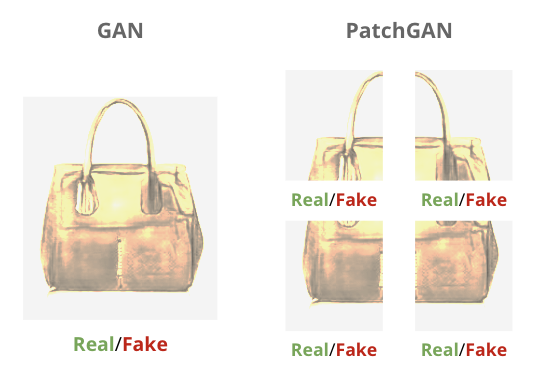
\includegraphics[width=0.6\hsize]{figure/patchgan.png}
\caption[通常のGANの識別モデルとPatchGANの比較]{通常のGANの識別モデルとPatchGANの比較\\
図は~\cite{pix2pix}のFigure~1を用いて作成した。}
\label{fig:patchgan}
\end{figure}

Pix2pixの識別モデルには、PatchGANという手法が用いられる。PatchGANは\prettyref{fig:patchgan}のように画像全体ではなくパッチと呼ばれる局所領域ごとに真偽を求めて平均を出力とする。これにより、局所的な識別精度が高まることが期待される。